%!TEX root = ../main.tex

\item Demuestra que la compactificación por un punto de $\mathbb{R}$ es homeomorfa al círculo $S^1$.\\

\begin{proof}
    Vamos a construir el homeomorfismo, este es la proyección estereográfica.

\begin{center}
    \tikzset{every picture/.style={line width=1.3pt}}

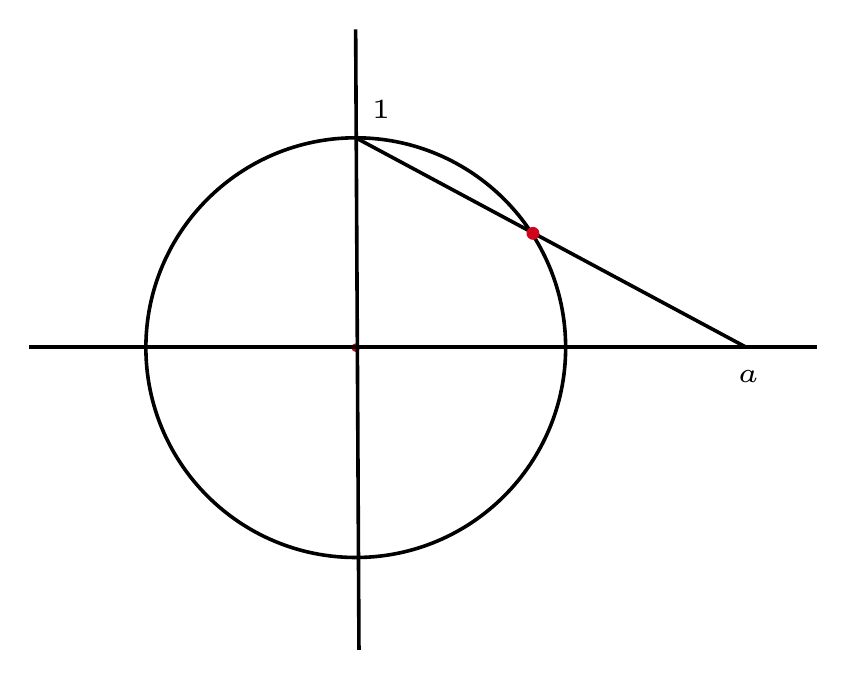
\begin{tikzpicture}[x=2pt,y=2pt,yscale=-1,xscale=1]
%uncomment if require: \path (0,300); %set diagram left start at 0, and has height of 300

%Shape: Ellipse [id:dp2076532777529081] 
\draw   (141.83,89.08) .. controls (141.83,68.14) and (158.81,51.17) .. (179.75,51.17) .. controls (200.69,51.17) and (217.67,68.14) .. (217.67,89.08) .. controls (217.67,110.02) and (200.69,127) .. (179.75,127) .. controls (158.81,127) and (141.83,110.02) .. (141.83,89.08) -- cycle ;
%Shape: Ellipse [id:dp49047118671320233] 
\draw  [draw opacity=0][fill={rgb, 255:red, 208; green, 2; blue, 27 }  ,fill opacity=1 ] (178.97,89.08) .. controls (178.97,88.65) and (179.32,88.3) .. (179.75,88.3) .. controls (180.18,88.3) and (180.53,88.65) .. (180.53,89.08) .. controls (180.53,89.52) and (180.18,89.87) .. (179.75,89.87) .. controls (179.32,89.87) and (178.97,89.52) .. (178.97,89.08) -- cycle ;
%Straight Lines [id:da9873077654790294] 
\draw    (179.73,31.6) -- (180.33,143.67) ;
%Straight Lines [id:da48767165474320806] 
\draw    (120.8,88.93) -- (263.13,88.93) ;
%Straight Lines [id:da6624476477384516] 
\draw    (179.75,51.17) -- (250.13,88.93) ;
%Shape: Circle [id:dp8959989266574702] 
\draw  [draw opacity=0][fill={rgb, 255:red, 208; green, 2; blue, 27 }  ,fill opacity=1 ] (210.6,68.43) .. controls (210.6,67.79) and (211.12,67.27) .. (211.77,67.27) .. controls (212.41,67.27) and (212.93,67.79) .. (212.93,68.43) .. controls (212.93,69.08) and (212.41,69.6) .. (211.77,69.6) .. controls (211.12,69.6) and (210.6,69.08) .. (210.6,68.43) -- cycle ;

% Text Node
\draw (181.2,43.07) node [anchor=north west][inner sep=0.75pt]  [font=\tiny,xscale=2,yscale=2]  {$1$};
% Text Node
\draw (247.33,91.82) node [anchor=north west][inner sep=0.75pt]  [font=\tiny,xscale=2,yscale=2]  {$a$};


\end{tikzpicture}
\end{center}


Por la ecuación de punto pendiente, la recta que se observa en el dibujo y que corta la circunferencia  tiene la ecuación 

$$y=\frac{-x}{a}+1,$$

reemplazando esto en la ecuación del círculo $(x^2+y^2=1)$obtenemos que 

$$x^2+\frac{x^2}{a^2}-\frac{2x}{a}=0,$$

así pues

$$x\left(1+\frac{1}{a^2}\right)=\frac{2}{a},$$

esto es 

$$x=\frac{2a}{a^2+1}.$$

Finalmente, al reemplazar $x$ en la ecuación de la recta, obtenemos que 

$$y=\frac{-2}{a^2+1}+1$$

que es el heomemorfimo ya que cuando $a\to \infty$ obtenemos el polo norte y la función establece una correspondencia entre un punto en la circunferencia y un punto en la recta (por la construcción que hicimos). Obviamente la función es biyectiva y continua y su inversa es continua xd.

\end{proof}

